\documentclass[letterpaper]{article}
\usepackage{natbib,alifexi}
\usepackage[utf8]{inputenc}
\usepackage{amsmath}
\usepackage[toc,page]{appendix}
\usepackage[frenchb]{babel}
\usepackage[T1]{fontenc}
\usepackage{placeins}

\title{Prédiction des temps de trajet dans un réseau\\ de bus à l'aide de données historiques}
\author{Nikita Marchant$^{1}$\\
Superviseurs : Martine Labbé, Samuel Deleplanque
\mbox{}\\\\
$^1$Université Libre de Bruxelles, Département d'Informatique\\
nimarcha@ulb.ac.be}

\setlength{\parskip}{0.5em}
\begin{document}
\maketitle

\begin{abstract}

\end{abstract}

\section{Introduction}

Le but de ce projet est de pouvoir prédire, en temps réel, l'heure d'arrivée d'un véhicule de transport en commun aux arrêts de son trajet.
Dans le cadre de ce travail, la prédiction sera effectuée pour des lignes de bus,
tram et métro de la STIB\footnote{Société de transports en commun à Bruxelles (Belgique)}.

Un réseau de transport en commun étant très difficile à modéliser à cause de sa complexité et par ce qu'il est très influençable par des événements stochastiques,
l'approche qui sera utilisée ici sera non pas de modéliser le réseau pour prédire son état futur mais d'extrapoler grâce à des algorithmes de machine learning les trajets des véhicules grâce à des données historiques récoltées au préalable.

\section{État de l'art}

\subsection{Méthodes naïves}

Plusieurs méthodes prédiction naïves de sont décrites dans la littérature, souvent pour servir de témoin et pouvoir comparer les performances de l'algorithme proposé par rapport aux méthodes naïves [\cite{Altinkaya2013}].

La plus simple des méthodes naïves est de prédire la durée de trajet entre deux arrêts en utilisant simplement la durée spécifiée dans les horaires statiques préparés par l'opérateur de la ligne. Cette méthode ne prenant aucun aléa en compte, elle n'est évidemment pas utilisée pour de la prédiction temps réel.

La seconde méthode, celle utilisée par la STIB, est de prédire le temps de trajet entre deux arrêts comme étant la moyenne des temps de trajets des $n$ (dans notre cas, 3) derniers véhicules de la ligne étant passés sur ce tronçon. Celle-ci donne malheureusement des résultats quasiment toujours moins bons que les autres méthodes existantes [\cite{Altinkaya2013}].

Un de ces points faibles est qu'elle est limitée par le fait qu'il faut attendre que $n$ véhicules aient subi une perturbation donnée pour qu'elle soit pleinement prise en compte pour les prédictions suivantes (et sur ce temps là, la perturbation sera peut-être finie).

Un autre problème dont souffre cette méthode est le fait qu'un bus peut se remplir fortement en une seule fois (par exemple à la sortie d'une école ou lors de la fin d'un gros événement). Celui-ci sera donc fortement ralenti à cause du temps pris à charger et décharger ses passagers alors que le modèle prédira qu'il sera aussi rapide que les véhicules précédents.

De plus, les véhicules qui suivent celui qui est retardé seront prédits en retard alors qu'ils risquent même d'être en avance, ayant moins de passagers à embarquer et débarquer.

Il existe aussi des méthodes hybrides comme celle présentée dans \cite{lin1999experimental} qui utilisent la position GPS, l'horaire statique ainsi que le retard calculé pour prédire l'heure d'arrivée. Celles-ci nécessitent des données plus précisent et d'une meilleure résolution mais donnent aussi de meilleurs résultats.



\subsection{Vitesse moyenne}

Comme le modèle hybride présenté ci-dessus, d'autres modèles exploitent le fait que certaines compagnies équipent leur véhicules de systèmes qui émettent en continu leur position GPS ainsi que leur vitesse. La position du véhicule n'étant évidement pas infiniment précise, il faut donc ensuite utiliser des techniques de \textit{map-matching} : faire correspondre le trajet mesuré au trajet prévu, sur une carte, afin de connaître sa ``vraie'' position.

Il est ensuite éventuellement possible de pouvoir transformer cette positions en deux dimensions en une position unidimensionnelle (la distance parcourue sur la ligne depuis le terminus) pour simplifier les algorithmes de prédiction.

Grâce à ces informations, il est possible d'estimer la vitesse du véhicule (le vitesse instantanée pouvant être nulle et donc prédire un temps d'attente infini, nous ne pouvons pas l'utiliser directement).

Pour cela, \cite{Maciver2002} combine la vitesse moyenne (calculée à l'aide des mesures précédentes) avec la vitesse instantanée rapportée par le véhicule. Le temps restant jusqu'à l'arrêt suivant est ensuite estimé comme la distance restant à parcourir multipliée par la vitesse.

\subsection{Régression}





\subsection{Filtres de Kalman}

Les filtres de Kalman [\cite{kalman1960new}] sont utilisés couramment dans la littérature [\cite{wall1999algorithm, cathey2003prescription, shalaby2004prediction}] pour leur fonction première : filtrer et lisser les mesures bruitées reçues depuis les véhicules. De plus, ceux-ci, de par leur fonctionnement interne permettent aussi d'estimer de l'état d'un système.
Dans notre cas, ils sont utilisés pour estimer l'état des véhicules, y compris leur vitesse et leur position.

En plus de cela, les filtres de Kalman peuvent aussi être utilisés pour de la prédiction et \cite{cathey2003prescription} sont les premiers à le faire pour prédire des temps d'arrivée de transports en commun et on été suivis par beaucoup d'autres (voir \cite{yang2005travel, Altinkaya2013}).

\cite{cathey2003prescription} ont montré que ceux-ci étaient meilleurs que les modèles basés sur des moyennes historiques et que ceux utilisant la régression. Cependant, ceux-ci ne prennent en compte qu'un trajet à la fois et ne profitent pas des données historiques pour apprendre des comportements récurrents.

\subsection{$k$ plus proches voisins}

La méthodes des $k$ plus proches voisins\footnote{$k$-nearest neighbors ou encore $k$-NN.} est une méthode largement utilisée dans le domaine des transports publics. Celle-ci prend
\subsection{SVM}

\subsection{ANN}




\section{Méthode développée}

Tous les réseaux urbains étant différents, les méthodes décrites dans l'état de l'art ne sont pas directement applicables à notre cas d'étude : le réseau de la STIB. Dans notre cas, nous ne disposons ni de trace GPS, ni d'information sur le taux de remplissage des véhicules ce qui élimine déjà une grande partie des méthodes présentées ci-dessus.

La méthode qui a été développée dans le cadre de ce travail est la méthode des $k$ plus proches voisins.

% TODO pourquoi knn

L'implémentation a été découpées en $n$ grandes parties : premièrement, la collection de données pour alimenter l'apprentissage du modèle, ensuite le traitement de ces données pour améliorer leur qualité et les transformer en un format utilisable par le modèle, l'étape suivante a été l'analyse et le choix de fonctions de score pour entraîner le modèle et pour finir, l’entraînement en lui même ainsi que l'analyse des résultats.

\subsection{Collection des données}

La STIB ne mettant pas à disposition ses données historiques, il a fallu commencer par récolter des informations grâce à un programme écrit pour l'occasion. Les deux seules sources de données sur l'état du réseau en temps réel disponibles sur internet sont : premièrement, pour chaque ligne, la position précise à un arrêt prêt de chaque véhicule et deuxièmement, pour chaque arrêt, une estimation du temps d'attente avant le prochain véhicule de chaque ligne.

La source de données qui a été choisie est la première pour deux raisons : le réseau de la STIB disposant de milliers d'arrêts, il aurait été difficile de récolter avec une fréquence suffisante les temps d'attente pour chaque arrêt. De plus, les temps d'attentes étant eux mêmes des prédictions, il serait un peu illogique de les utiliser comme des mesures.

La source choisie souffre tout de même d'un problème non-négligeable : les véhicules apparaissent sur la ligne comme de simples point non identifiés. Il n'est donc pas possible de récupérer le numéro du véhicule, sa plaque d'immatriculation ou tout autre identifiant unique. De plus, si deux véhicules d'une même ligne sont suffisamment proches, ils n'apparaissent plus que comme un seul point.

Le processus de collection des données est un programme \textit{Python3} utilisant \texttt{aiohttp} pour permettre des requêtes http asynchrones au serveur web de la STIB et ainsi permettre une période d’échantillonnage de 20 secondes pour chaque ligne, dans chaque sens (ce qui fait 142 mesures toutes les 20 secondes dans l'état actuel du réseau). La période a été choisie arbitrairement car une fréquence plus élevée imposait une charge trop lourde au serveur de le STIB et une fréquence plus faible aurait été trop imprécise.

Cette collection de données a permis l'enregistrement d'approximativement 80 millions de mesures en 6 mois, réparties sur l'ensemble des lignes.


\subsection{Traitement des données}

Les données récupérées grâce à la méthode décrite dans la section précédente sont malheureusement de mauvaise qualité : il est courant qu'un véhicule cesse d’émettre sa position pendant plusieurs minutes, que la source de donnée tombe en panne ou que les positions de deux véhicules fort proches soient confondues en un seul point.

De plus, les mesures ne sont pas directement utilisables par l'algorithme que nous avons choisi. En effet, nous ne disposons que d'une suite de positions (les sorties de notre programme de mesure sont des vecteurs horodatés de booléens, voir annexes) et ce dont nous avons besoin est des durées que chaque véhicule a pris pour parcourir les distances entre deux arrêts consécutifs.

Nous avons donc développé un algorithme qui assigne un identifiant à chaque nouveau point qui apparaît sur une ligne et qui essaye, dans la mesure du possible, de détecter lors des mesures suivantes si un point est déjà connu et qu'il s'est déplacé ou si c'est un nouveau point (par exemple un bus qui vient du dépôt).

Grâce à ces identifiants, nous pouvons donc maintenant reconstituer des trajets (une suite de paires [position, instant]) pour ces véhicules en parcourant les mesures et en enregistrant la position de chaque identifiant dans la ligne à chaque instant.

Dans l'optique de pouvoir proposer des prédictions en temps réel, l'algorithme supporte un mode dans lequel il a connaissance des trajets passés dont le véhicule n'est pas arrivé au terminus et qui permet de compléter ces trajets au fur et à mesure que de nouvelles mesures sont disponibles.

L'algorithme, bien qu'ayant pris du temps à développer et à paramétrer ne présente pas de grand intérêt scientifique. Son fonctionnement est donc décrit en annexe.

\subsection{Modèle d'apprentissage: les $k$ plus proches voisins}

L'algorithme des $k$ plus proches voisins
est une méthode d'intelligence artificielle qui peut être utilisée aussi bien pour de la classification que pour de la régression [\cite{trevor2009elements}].
L'idée de cette méthode est de trouver les $k$ trajets les plus similaires à la cible et d'utiliser ceux-ci pour extrapoler le temps de trajet futur.

Pour calculer la similarité entre deux trajets, nous devons extraire des \textit{features}, des grandeurs qui caractérisent ces trajets. Les features que nous utiliserons ici sont les temps que le véhicule a pris pour voyager entre deux arrêts. Un trajet n'est évidemment pas caractérisé uniquement par ces grandeurs mais nous verrons qu'en première approximation ces grandeurs sont déjà suffisantes \footnote{Une autre feature très intéressante et fort utilisée dans la littérature est la taux de remplissage du véhicule mais nous n'avons pas accès à cette donnée dans notre cas. D'autres features qui pourraient être intéressantes sont énumérées dans les perspectives, en fin d'article}.

Pour cela, nous projetons chaque trajet dans un espace à $n$ dimensions avec $n+1$ étant le nombre d'arrêts déjà effectués par le véhicule dont on cherche à prédire le temps de trajet (ce véhicule sera appelé $\alpha$).

Les trajets sont donc représentés par le vecteur colonne
$T_{\alpha} = \begin{pmatrix}d_{1,\beta}, d_{2,\beta}, ..., d_{n,\beta}\end{pmatrix}^{T}$
avec $d_{i,\beta}$ étant la durée du trajet entre l'arrêt $i$ et $i+1$ pour le véhicule $\beta$.

Maintenant que nous avons transformé nos trajets en vecteurs, nous pouvons utiliser tous les trajets du passés (l'ensemble d'apprentissage) et les placer dans cet espace à $n$ dimensions pour entraîner notre algorithme.

Une fois que l'algorithme est entraîné, nous pouvons faire une prédiction pour un nouveau trajet ($\hat{d}$) dont on ne connaît pas la fin. Pour cela, nous le plaçons aussi dans cet espace et nous mesurons sa similarité par rapport à tous les autres trajets de l'ensemble d'apprentissage.

La similarité $s_{\alpha,\beta}$ (ou distance) entre deux trajets $\alpha$ et $\beta$ est définie comme la distance euclidienne entre deux vecteurs :

\begin{eqnarray}
s_{\alpha,\beta} = \sqrt{\sum_{j=0}^{n}(d_{j,\alpha} - d_{j,\beta})^2}
\end{eqnarray}

Nous sélectionnons ensuite les $k$ vecteurs dont la similarité est la plus proche de $\hat{d}$ et nous nommons cet ensemble $\mathcal{V}$ : les plus proches voisins.

Dans la version originale de $k$NN, la prédiction du temps de trajet $\hat{d}_{n+1,\alpha}$ est ensuite donnée par la moyenne des temps de trajets pour les vecteur appartenant à $\mathcal{V}$.

\begin{eqnarray}
\hat{d}_{n+1,\alpha} = \frac{1}{k} \sum_{i \in \mathcal{V}}d_{n+1,i}
\end{eqnarray}

Il est aussi possible d'effectuer la régression à l'aide d'une moyenne pondérée. Chaque vecteur est pondéré par l'inverse de sa distance par rapport au vecteur cible :

\begin{eqnarray}
\hat{d}_{n+1,\alpha} = \sum_{i \in \mathcal{V}} s_{\alpha, i} \cdot \frac{1}{k} \sum_{i \in \mathcal{V}}( \frac{d_{n+1,i}}{s_{\alpha, i}})
\end{eqnarray}

La projection des trajets dans un espace à $n$ dimension ainsi que l'implémentation de l'algorithme des plus proches voisin ont dans un premier temps été écrits en \textit{Python3}, uniquement à l'aide de la librairie \texttt{numpy} pour faciliter les calculs vectoriels et un prototypage rapide. Dans un second temps, nous avons utilisé la librairie \texttt{scikit-learn} pour profiter de son implémentation optimisée de $k$NN.

\section{Fonctions de score}

Afin d'effectuer un bon choix de l'hyper-paramètre $k$ ainsi que de choisir entre la moyenne pondérée ou non, il est important de pouvoir comparer deux modèles entre eux. Pour cela, nous aurons aussi besoin d'assigner un score à une prédiction en fonction de sa performance par rapport à ce qu'il c'est vraiment passé.

\subsection{Score d'une prédiction}
Pour assigner un score à une prédiction, la littérature utilise souvent le RMSE\footnote{Root Mean Squared Error}: l'erreur quadratique moyenne.
Cependant, cette métrique souffre d'un problème :
qu'un bus soit annoncé une minute à l'avance ou une minute en retard est pondéré de la même manière alors que dans un cas l'usager attend son bus une minute de plus et que dans l'autre il le rate.

Nous avons donc implémenté d'autres métriques qu'il nous semblait intéressant de pouvoir minimiser :
\begin{itemize}
    \item Le RMSE double négatif : chaque erreur négative (quand un bus est annoncé plus tard qu'en vrai) est doublée et en suite on applique le RMSE.
    \item RMSE pondéré linéairement : l'erreur de prédiction pour l'arrêt suivant est pondéré avec un poids de 5, l'erreur pour le dernier arrêt est pondérée avec un poids de 1 et les arrêts entre les deux sont pondérés linéairement entre 1 et 5.
    \item RMSE pondéré exponentiellement : l'erreur de prédiction pour le $n$ème arrêt est pondéré avec un poids de $\frac{1}{n}$
\end{itemize}
\vspace{1em}

La première métrique résout (ou en tout cas diminue) le problème du bus raté et les deux suivantes prennent en compte le fait qu'il est plus intéressant de bien prédire le futur proche et un peu moins bien le futur lointain que de bien prédire l'entièreté du trajet.

Avant de choisir la métrique que nous utiliserons comme fonction de score, nous avons décidé de les comparer.
Pour cela, nous entraîné un $k$NN avec un $k$ fixé arbitrairement à 130 à l'aide de 12000 trajets de la ligne de bus 95 vers Grand-Place en utilisant les 10 premiers arrêts comme donnée connue et les 13 suivants comme donnée à prédire. Ensuite, nous avons effectué 6000 prédictions pour d'autres trajets de la même ligne et nous avons calculé leur score avec chaque métrique.

\begin{figure}
   \centerline{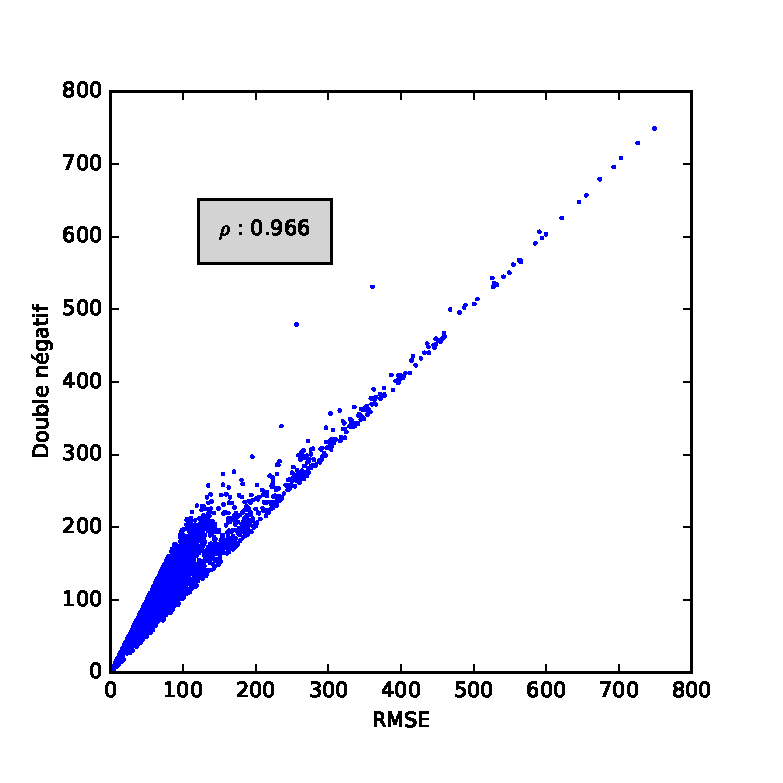
\includegraphics[width=8cm]{metrics.eps}}
   \caption{\label{fig:rmse-vs-double}Comparaison entre le RMSE et le double négatif pour chacune des prédictions.}
\end{figure}

Nous avons ensuite comparé graphiquement deux à deux chacune des fonctions de score sur l'ensemble des 6000 prédictions. Nous pouvons en voir un exemple dans la figure~\ref{fig:rmse-vs-double} : chaque point représente une prédiction avec, en l’abscisse son score selon le RMSE et en ordonnée son score selon le RMSE double négatif. Des graphes pour toutes les autres comparaisons se trouvent en annexe.

Cette première comparaison nous a déjà permis d'apercevoir une corrélation linéaire entre les différentes fonctions.
En plus de cette corrélation déterminée visuellement, nous avons comparé la corrélation de rang entre les fonctions grâce au coefficient de corrélation de Spearman (ou $\rho$). Celui-ci nous donne un indice sur le fait que deux fonctions ordonnent un ensemble de la même manière\footnote{En effet, il nous importe peu que la corrélation soit linéaire ou même quadratique : tant qu'on peut classer les prédiction de la meilleure à la moins bonne et que ce classement ne change pas lors d'un changement de fonction de score, cela est suffisant pour nous.}. Celui-ci varie entre -1, quand l'ordre est parfaitement inversé à 1, quand l'ordre est identique.

Sa formule est définie comme ceci, $d$ étant la différence entre le rang défini par la première fonction et celui défini par la seconde :

\begin{eqnarray}
\rho = 1 - \frac{6 \sum_{i=1}^{n} d^2_i}{n^3 - n}
\end{eqnarray}

\begin{table}[h]
\centering
\begin{tabular}{|l|c|c|c|c|}
  \hline
  & RMSE & linéaire & exponentiel & double \\
  \hline
RMSE & 1.000 & 0.961 & 0.812 & 0.966 \\
linéaire & 0.961 & 1.000 & 0.896 & 0.926 \\
exponentiel & 0.812 & 0.896 & 1.000 & 0.793 \\
double & 0.966 & 0.926 & 0.793 & 1.000 \\
  \hline
\end{tabular}
  \caption{\label{tab:rho} Rho de Spearman entre chaque chaque paire de métrique de score.}
\end{table}

Le RMSE double négatif semblant être la métrique la plus intéressante à minimiser pour les utilisateurs et le RMSE simple étant quasiment identique (voir table \ref{tab:rho} et figure \ref{fig:rmse-vs-double}), nous avons choisi d'utiliser par la suite le RMSE pour sa simplicité d'implémentation et sa rapidité (ce n'est que la norme du vecteur d'erreur, fonction qui est déjà implémentée rapidement dans \texttt{numpy})

\FloatBarrier
\subsection{Score d'une modèle}

Maintenant que nous savons comparer et donner un score à des prédictions, nous pouvons choisir une technique pour scorer un modèle en entier, ce qui nous permettra entre autres de choisir l'hyper-paramètre $k$ et de choisir entre le $k$NN pondéré ou non.

Pour cela, nous devons agréger d'une manière ou d'une autres toutes les prédiction qu'un modèle a fait pour un ensemble de départ. Ici le choix des fonctions d’agrégation score ont été assez simples. Nous avons comparé la moyenne, la médiane ainsi que le maximum de l'ensemble des scores des prédictions du modèle.

Pour cela, nous avons réutilisé le même set de données que dans la section précédente mais cette fois ci en faisant varier $k$ de 1 à 1000 en 20 incréments\footnote{Nous avons peu d’échantillons par rapport à la comparaison précédente car il est coûteux computationnellement de créer, entraîner et scorer des centaines de modèles.}.

Nous avons remarqué une corrélation assez forte, 0.822, entre la médiane et la moyenne ainsi qu'une absence totale de corrélation entre le maximum et les deux autres (0.007 et 0.180).

Cela semblerait s'expliquer par le fait que même si un modèle est très précis la plus part du temps, il fera tout de même au moins une grosse erreur et que cette erreur est bornée supérieurement par la distance entre le trajet le plus lent et le plus rapide.

Au vu de la faible différence entre la moyenne et la médiane, mous avons arbitrairement choisi d'utiliser la moyenne comme fonction d'agrégation de scores.

Pour éviter l'\textit{overfitting} (en français le sur-apprentissage), le fait qu'un modèle donne des résultats artificiellement bons pour l'ensemble d’entraînement au détriment de bonnes prédictions pour de nouveaux échantillons, nous avons utilisé la méthode de la validation croisée.

La validation croisée (ou plus communément \textit{cross-validation}) est une technique qui permet d'estimer la fiabilité d'un modèle grâce à un échantillonnage des données. Nous avons utilisé la méthode \textit{testset validation} pour des raisons de complexité computationnelle.

Cette méthode fonctionne de la manière suivante : l'ensemble des trajets divisé en deux échantillons, l'un contenant $2/3$ des données et le second contenant le dernier tiers. Le premier devient l'ensemble d'apprentissage et sert uniquement à entraîner le modèle alors que le second devient l'ensemble de test et dont les prédictions serviront à scorer le modèle.

\subsection{Entraînement et choix des paramètres}

Une fois les méthodes de score déterminées, nous pouvons choisir expérimentalement une valeur pour l'hyper-paramètre $k$ en cherchant à minimiser le score de notre modèle.

Nous voyons empiriquement que quand $k$ augmente, le score d'un modèle diminue de manière presque continue jusqu'à atteindre le $k$ optimal puis se mets à augmenter une fois ce point dépassé.

Au lieu d'itérer sur l'entièreté des valeurs possible de $k$ (par exemple l’intervalle $[1,1000]$) pour trouver la valeur minimale de $f(k)$, nous avons utilisé la méthode de Brent, décrite dans \cite{rivlin1973algorithms}, détaillée en annexe et implémentée dans \texttt{scipy} qui permet de minimiser une fonction dont l'expression analytique (et donc la dérivée) n'est pas connue.

Nous avons donc utilisé la méthode de Brent avec un nombre d'itérations limité à 40 et dont la convergence est considérée comme atteinte quand l'erreur relative est inférieure à 0,1.

Les résultats que nous avons obtenu sont des $k$ variant entre 100 et 800, selon les lignes. Le fait que c'est intervalle soit si large semble s'expliquer par le fait que chaque ligne à une fréquence différente et que par exemple, pour une ligne importante comme le 95 nous disposons de plus de 35000 trajets alors que pour une ligne à faible fréquence comme le 41 nous ne disposons que de 8000 trajets\footnote{Les mesures dont nous disposons pour les lignes à haute fréquence sont aussi de moins bonne qualité (il y a plus de chances que notre algorithme confonde deux véhicules ou ne détecte pas un dépassement quand les véhicules sont proches les uns des autres).}.

Nous avons ensuite effectué la même recherche de l'hyper-paramètre $k$ pour la version pondérée par la distance de $k$NN. Celle-ci a retourné approximativement les les mêmes $k$ optimaux, cependant la valeur de la fonction de score était systématiquement égale ou inférieure à la version non pondérée. Dans le cas de la ligne du 95, nous avons été jusqu'à constater un score deux fois meilleur pour la version pondérée.

\section{Résultats}

Le choix d'un hyper-paramètre permettant de minimiser l'erreur de prédiction nous permet maintenant de comparer nos prédictions faites à l'aide d'un $k$NN à celles faites par la STIB avec la méthode de la moyenne des trois derniers trajets.

Pour cela, nous avons utilisé la même méthode échantillonnage que précédemment. Nous avons donc entraîné notre modèle avec $2/3$ des données et effectué des prédictions sur le tiers restant (l'ensemble de test). Ensuite, pour chaque trajet de l'ensemble de test, nous cherché les trois trajets précédents dans le temps (qu'ils appartiennent à l'ensemble de test ou non) pour en faire la moyenne et l'utiliser comme la prédiction que la STIB aurait faite.

Les résultats démontrent l'efficacité de la méthode employée : pour certaines lignes, notre modèle prédit mieux que la STIB dans 75\% des cas.

\begin{table}[h]
\centering
\begin{tabular}{|l|c|c|c|c|}
  \hline
  & Ligne 5 & Ligne 41 & Ligne 95 \\
  \hline
  meilleur &  76\%  & 70\%  & 63\%  \\
  2x meilleur &  10\%  & 16\%  & 12\%  \\
  2x pire &  0.5\% & 0.6\% & 0.8\% \\
  \hline
\end{tabular}
  \caption{\label{tab:perf}Taux de réussite de notre modèle en fonction de la performance désirée}
\end{table}


De plus, on peut remarquer que lorsque que notre modèle se trompe plus que la STIB, ce n'est que de peu : $k$NN effectue une prédiction deux fois moins bonne que la STIB seulement dans 0.5\% des cas pour la ligne 5 (contre 10\% des cas pour des prédictions 2 fois meilleures). On peut observer\footnote{Des résultats pour d'autres lignes ainsi que d'autres visualisations de ceux-ci peuvent être trouvés en annexe} ce phénomène dans le tableau \ref{tab:perf} pour certaines valeurs cibles ou de manière générale dans la figure \ref{fig:heatmap}.

\begin{figure}[h]
   \centerline{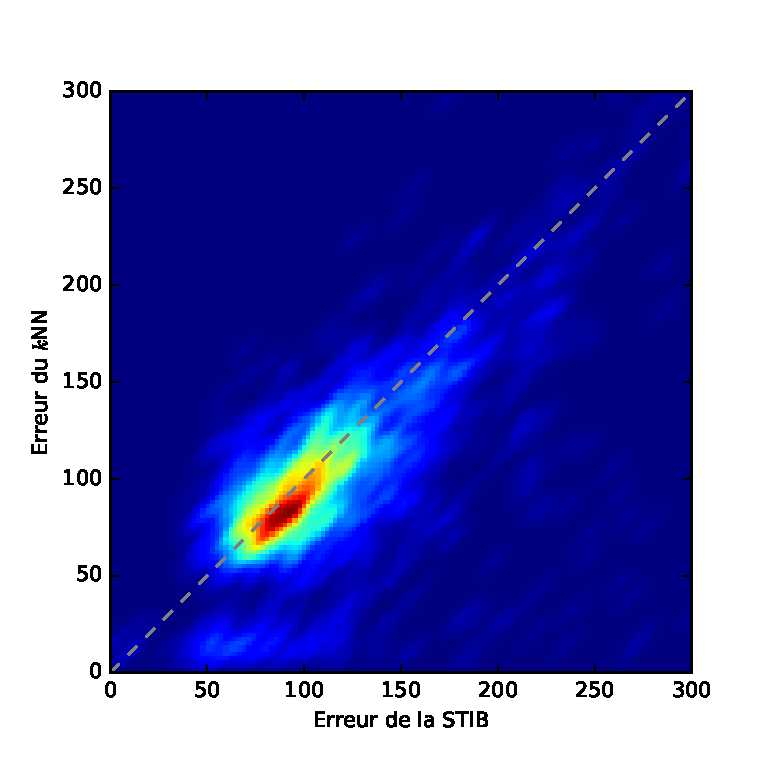
\includegraphics[width=8cm]{error-heatmap.eps}}
   \caption{\label{fig:heatmap} Estimation de la densité des trajets en fonction des erreurs de leurs prédictions selon le $k$NN ou la STIB pour la ligne 95. La ligne pointillée représente une erreur identique pour les deux modèles.}
\end{figure}



\section{Conclusion et perspectives}

Ce projet m'a permis d'apprendre énormément dans le domaine du machine learning ainsi que de proposer un modèle meilleur que l'actuel à la STIB pour leur prédiction en temps réel.

Ce travail pourrait être continué et amélioré soit en explorant d'autres méthodes d'apprentissage automatique comme les réseaux de neurones, la régression à l'aide de noyaux ou encore les ``support vector machines'' qui ont l'air prometteurs.

En restant dans le domaine des $k$ plus proches voisins. Plusieurs pistes sont explorables :
actuellement mon modèle ne prend en compte que les temps de trajet entre les arrêts dans le passé pour chaque bus.
Il serait intéressant d'ajouter d'autres variables comme la distance du bus par rapport au bus qui le précède, l'heure de la journée, le jour de la semaine, le type de jour (férié, vacances, ...), des variables météorologiques, la longueur des embouteillages dans la ville,~...

Pour finir, il serait aussi intéressant d'améliorer la qualité et la précision des données en entrée de l'algorithme, que ce soit par une meilleure imputation des données manquantes ou par une source de meilleure qualité car il y a de fortes chances que des données de meilleure qualité permettent des prédictions plus justes.

\footnotesize
\bibliographystyle{apalike}
\bibliography{example}


\newpage
\begin{appendices}
\section{Algorithmes de traitement et de collection de données}
\subsection{Source de données}
\label{align}
Notre source primaire de donnés se présente comme ceci :

\begin{figure}[h]
   \centerline{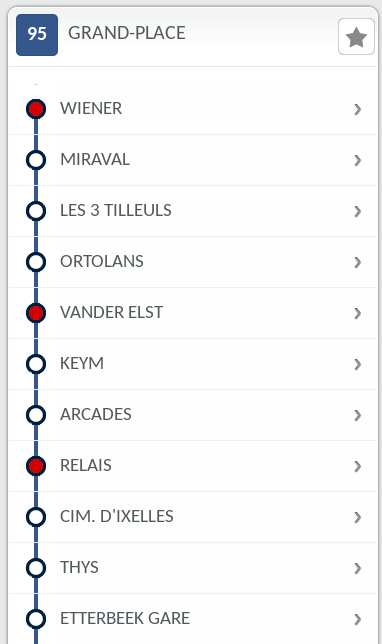
\includegraphics[width=3cm]{mstib.png}}
\end{figure}

Chaque point rouge représentant au minimum un véhicule (mais parfois plus dans le cas ou ils seraient trop proches les uns des autres). La mesure correspondant à cette copie d'écran serait ceci (un vecteur de booléens) : \texttt{[vrai, faux, faux, faux, vrai, faux, faux, vrai, faux, faux]}

\subsection{Problèmes rencontrés}

\subsection{Description du fonctionnement}

\subsection{Imputation des données manquantes}

Une fois ce traitement effectué, il reste un dernier détail à prendre en compte : les trajets extraits ne commencent ou ne finissent pas tous au terminus (soit parce que le véhicule n'as pas été jusqu'au bout ou à cause d'erreurs commises lors de l'extraction des trajets depuis les positions).

Les méthodes présentées ci-dessus ne fonctionnant pas avec des vecteurs contenant des éléments non définis, il y avait deux possibilités : soit ignorer les vecteurs incomplets soit extrapoler les valeurs manquantes.

La première méthode a été écartée car elle diminuait fortement la taille de l'ensemble d'apprentissage, la seconde a été privilégiée. Si le $i$ème élément d'un vecteur est manquant, il est remplacé par la moyenne des $i$èmes éléments des vecteurs dont la valeur est définie.



\section{Méthode de Brent}

\section{Résultats}


\end{appendices}

\end{document}
